%\RequirePackage[l2tabu, orthodox]{nag}
\RequirePackage{currfile}
\documentclass[12pt]{beamer}
\graphicspath{{Imagenes/}{../Imagenes/}}
\usepackage[utf8]{inputenc}
\usepackage[spanish]{babel}
\usepackage{standalone}
\usepackage{color}
\usepackage[binary-units=true]{siunitx}
\usepackage{hyperref}
\hypersetup{
  colorlinks=true,
  linkcolor=blue,          % color of internal links (change box color with linkbordercolor)
  citecolor=green,        % color of links to bibliography
  filecolor=magenta,      % color of file links
  urlcolor=cyan,           % color of external links
  linkbordercolor={0 0 1}
}
\usepackage{xcolor, soul}
\usepackage{etoolbox}
\usepackage{amsmath}
\usepackage{amsthm}
\usepackage{physics}
\usepackage{multicol}
\usepackage{graphicx}
\usepackage{bookmark}
\usepackage{longtable}
\usepackage{graphicx}
\usepackage{tikz}
\usepackage[siunitx, RPvoltages]{circuitikz}
\usetikzlibrary{mindmap}
\usetikzlibrary{arrows, patterns, shapes, decorations.markings, decorations.pathmorphing}
\usetikzlibrary{matrix,positioning}
\tikzstyle{every picture}+=[remember picture,baseline]
\usepackage[autostyle,spanish=mexican]{csquotes}
\usepackage{pifont}
\usepackage[font=footnotesize,textfont=it]{caption}
\usepackage{tabulary}
\usepackage{booktabs}
\usepackage[outdir=./]{epstopdf}
%\usepackage{epstopdf}
\usepackage{media9}
\usepackage{multimedia}
\usepackage{bigints}
%\usepackage{enumitem}
\usepackage[os=win]{menukeys}
\usepackage{pifont}
\usepackage{pbox}
\usepackage{alltt}
\usepackage{verbatim}
\usepackage{colortbl}
\usepackage{tcolorbox}
\usepackage{fancyvrb}
\usepackage[sfdefault]{roboto}  %% Option 'sfdefault' only if the base font of the document is to be sans serif
%\usepackage[T1]{fontenc}
\setcounter{secnumdepth}{3}
\setcounter{tocdepth}{3}
\DeclareGraphicsExtensions{.pdf,.png,.jpg}
\renewcommand {\arraystretch}{1.5}
\definecolor{ao}{rgb}{0.0, 0.5, 0.0}
\definecolor{aquamarine}{rgb}{0.5, 1.0, 0.83}
\definecolor{kellygreen}{rgb}{0.3, 0.73, 0.09}
\definecolor{bisque}{rgb}{1.0, 0.89, 0.77}
\definecolor{amber}{rgb}{1.0, 0.75, 0.0}
\definecolor{armygreen}{rgb}{0.29, 0.33, 0.13}
\definecolor{alizarin}{rgb}{0.82, 0.1, 0.26}
\definecolor{cadetblue}{rgb}{0.37, 0.62, 0.63}
\newcommand*{\TitleParbox}[1]{\parbox[c]{6cm}{\raggedright #1}}%
\newcommand{\python}{\texttt{python}}
\newcommand{\textoazul}[1]{\textcolor{blue}{#1}}
\newcommand{\azulfuerte}[1]{\textcolor{blue}{\textbf{#1}}}
\newcommand{\funcionazul}[1]{\textcolor{blue}{\textbf{\texttt{#1}}}}
%\normalfont
\usepackage{ccfonts}% http://ctan.org/pkg/{ccfonts}
\usepackage[T1]{fontenc}% http://ctan.or/pkg/fontenc
\renewcommand{\rmdefault}{cmr}% cmr = Computer Modern Roman
\usefonttheme[onlymath]{serif}
\linespread{1.3}
\newcounter{saveenumi}
\newcommand{\seti}{\setcounter{saveenumi}{\value{enumi}}}
\newcommand{\conti}{\setcounter{enumi}{\value{saveenumi}}}
\newcommand{\tikzmark}[1]{\tikz[remember picture] \node[coordinate] (#1) {#1};}

\usepackage{scalerel}[2016-12-29]
\def\stretchint#1{\vcenter{\hbox{\stretchto[440]{\displaystyle\int}{#1}}}}
\def\scaleint#1{\vcenter{\hbox{\scaleto[3ex]{\displaystyle\int}{#1}}}}
\def\bs{\mkern-12mu}

\newtheorem{teo}{}[section]
\usepackage{blkarray}

%reduce el tamaño de letra de la etiqueta equations
\makeatletter
\def\maketag@@@#1{\hbox{\m@th\normalfont\small#1}}
\makeatother

%se usa para la x en itemize
\newcommand{\xmark}{\text{\ding{55}}}

%\AtBeginDocument{\setlength{\tymin}{1em}}


\definecolor{myblue}{rgb}{.8, .8, 1}

\usepackage{empheq}

\newlength\mytemplen
\newsavebox\mytempbox

\makeatletter
\newcommand\mybluebox{%
    \@ifnextchar[%]
       {\@mybluebox}%
       {\@mybluebox[0pt]}}

\def\@mybluebox[#1]{%
    \@ifnextchar[%]
       {\@@mybluebox[#1]}%
       {\@@mybluebox[#1][0pt]}}

\def\@@mybluebox[#1][#2]#3{
    \sbox\mytempbox{#3}%
    \mytemplen\ht\mytempbox
    \advance\mytemplen #1\relax
    \ht\mytempbox\mytemplen
    \mytemplen\dp\mytempbox
    \advance\mytemplen #2\relax
    \dp\mytempbox\mytemplen
    \colorbox{myblue}{\hspace{1em}\usebox{\mytempbox}\hspace{1em}}}

\makeatother



%Se usa la plantilla Warsaw modificada con spruce
\mode<presentation>
{
  \usetheme{Warsaw}
  \setbeamertemplate{headline}{}
  \useoutertheme{default}
  %\usecolortheme{beaver}
  \setbeamercovered{invisible}
}
%\AtBeginSection[]
%{
%\begin{frame}<beamer>{Contenido}
%\normalfont\mdseries
%\tableofcontents[currentsection]
%\end{frame}
%}

\setbeamertemplate{section in toc}[sections numbered]
\setbeamertemplate{subsection in toc}[subsections numbered]
\setbeamertemplate{subsection in toc}{\leavevmode\leftskip=3.2em\rlap{\hskip-2em\inserttocsectionnumber.\inserttocsubsectionnumber}\inserttocsubsection\par}
\setbeamercolor{section in toc}{fg=blue}
\setbeamercolor{subsection in toc}{fg=blue}
\setbeamertemplate{navigation symbols}{}
\setbeamercolor{frametitle}{fg=yellow,bg=blue!70!white}
\setbeamercolor{section in head/foot}{bg=gray!30,fg=red}
%\setbeamercolor{section in head}{bg=green,fg=red}
\setbeamercolor{subsection in head/foot}{bg=gray!30,fg=black}
\setbeamercolor{author in head/foot}{bg=gray!30}
\setbeamercolor{date in head/foot}{fg=blue}

%\mode<presentation>
%{
%  \usetheme{Warsaw}
%  \setbeamertemplate{headline}{}
%  %\useoutertheme{infolines}
%  \useoutertheme{default}
%  \setbeamercovered{invisible}
%  % or whatever (possibly just delete it)
%}

\usepackage{courier}
\usepackage{listingsutf8}
\usepackage{listings}
\usepackage{xcolor}
\usepackage{textcomp}
\usepackage{color}
\definecolor{deepblue}{rgb}{0,0,0.5}
\definecolor{brown}{rgb}{0.59, 0.29, 0.0}
\definecolor{OliveGreen}{rgb}{0,0.25,0}
% \usepackage{minted}

\DeclareCaptionFont{white}{\color{white}}
\DeclareCaptionFormat{listing}{\colorbox{gray}{\parbox{0.98\textwidth}{#1#2#3}}}
\captionsetup[lstlisting]{format=listing,labelfont=white,textfont=white}
\renewcommand{\lstlistingname}{Código}


\definecolor{Code}{rgb}{0,0,0}
\definecolor{Keywords}{rgb}{255,0,0}
\definecolor{Strings}{rgb}{255,0,255}
\definecolor{Comments}{rgb}{0,0,255}
\definecolor{Numbers}{rgb}{255,128,0}

\makeatletter

\newif\iffirstchar\firstchartrue
\newif\ifstartedbyadigit
\newif\ifprecededbyequalsign

\newcommand\processletter
{%
  \ifnum\lst@mode=\lst@Pmode%
    \iffirstchar%
        \global\startedbyadigitfalse%
      \fi
      \global\firstcharfalse%
    \fi
}

\newcommand\processdigit
{%
  \ifnum\lst@mode=\lst@Pmode%
      \iffirstchar%
        \global\startedbyadigittrue%
      \fi
      \global\firstcharfalse%
  \fi
}

\lst@AddToHook{OutputOther}%
{%
  \lst@IfLastOtherOneOf{=}
    {\global\precededbyequalsigntrue}
    {}%
}

\lst@AddToHook{Output}%
{%
  \ifprecededbyequalsign%
      \ifstartedbyadigit%
        \def\lst@thestyle{\color{orange}}%
      \fi
    \fi
  \global\firstchartrue%
  \global\startedbyadigitfalse%
  \global\precededbyequalsignfalse%
}

\lstset{ 
language=Python,                % choose the language of the code
basicstyle=\footnotesize\ttfamily,       % the size of the fonts that are used for the code
numbers=left,                   % where to put the line-numbers
numberstyle=\scriptsize,      % the size of the fonts that are used for the line-numbers
stepnumber=1,                   % the step between two line-numbers. If it is 1 each line will be numbered
numbersep=5pt,                  % how far the line-numbers are from the code
backgroundcolor=\color{white},  % choose the background color. You must add \usepackage{color}
showspaces=false,               % show spaces adding particular underscores
showstringspaces=false,         % underline spaces within strings
showtabs=false,                 % show tabs within strings adding particular underscores
frame=single,   		% adds a frame around the code
tabsize=2,  		% sets default tabsize to 2 spaces
captionpos=t,   		% sets the caption-position to bottom
breaklines=true,    	% sets automatic line breaking
breakatwhitespace=false,    % sets if automatic breaks should only happen at whitespace
escapeinside={\#},  % if you want to add a comment within your code
stringstyle =\color{OliveGreen},
%otherkeywords={{as}},             % Add keywords here
keywordstyle = \color{blue},
commentstyle = \color{black},
identifierstyle = \color{black},
literate=%
         {á}{{\'a}}1
         {é}{{\'e}}1
         {í}{{\'i}}1
         {ó}{{\'o}}1
         {ú}{{\'u}}1
%
%keywordstyle=\ttb\color{deepblue}
%fancyvrb = true,
}

\lstdefinestyle{FormattedNumber}{%
    literate={0}{{\textcolor{red}{0}}}{1}%
             {1}{{\textcolor{red}{1}}}{1}%
             {2}{{\textcolor{red}{2}}}{1}%
             {3}{{\textcolor{red}{3}}}{1}%
             {4}{{\textcolor{red}{4}}}{1}%
             {5}{{\textcolor{red}{5}}}{1}%
             {6}{{\textcolor{red}{6}}}{1}%
             {7}{{\textcolor{red}{7}}}{1}%
             {8}{{\textcolor{red}{8}}}{1}%
             {9}{{\textcolor{red}{9}}}{1}%
             {.0}{{\textcolor{red}{.0}}}{2}% Following is to ensure that only periods
             {.1}{{\textcolor{red}{.1}}}{2}% followed by a digit are changed.
             {.2}{{\textcolor{red}{.2}}}{2}%
             {.3}{{\textcolor{red}{.3}}}{2}%
             {.4}{{\textcolor{red}{.4}}}{2}%
             {.5}{{\textcolor{red}{.5}}}{2}%
             {.6}{{\textcolor{red}{.6}}}{2}%
             {.7}{{\textcolor{red}{.7}}}{2}%
             {.8}{{\textcolor{red}{.8}}}{2}%
             {.9}{{\textcolor{red}{.9}}}{2}%
             {\ }{{ }}{1}% handle the space
         ,%
          %mathescape=true
          escapeinside={__}
          }



\makeatletter
\setbeamertemplate{footline}
{
  \leavevmode%
  \hbox{%
  \begin{beamercolorbox}[wd=.333333\paperwidth,ht=2.25ex,dp=1ex,center]{author in head/foot}%
    \usebeamerfont{author in head/foot} \insertsection
  \end{beamercolorbox}}%
  \begin{beamercolorbox}[wd=.333333\paperwidth,ht=2.25ex,dp=1ex,center]{title in head/foot}%
    \usebeamerfont{title in head/foot} \insertsubsection
  \end{beamercolorbox}%
  \begin{beamercolorbox}[wd=.333333\paperwidth,ht=2.25ex,dp=1ex,right]{date in head/foot}%
    \usebeamerfont{date in head/foot} \textcolor{white}{\insertshortdate{}} \hspace*{2em}
    \textcolor{white}{\insertframenumber{} / \inserttotalframenumber}\hspace*{2ex} 
  \end{beamercolorbox}}%
  \vskip0pt%
\makeatother
\title{\large{Tema 1 - Escalas, condición y estabilidad}}
\subtitle{Curso de Física Computacional}
\author[]{M. en C. Gustavo Contreras Mayén}
\date{\today}
\institute{Facultad de Ciencias - UNAM}
\titlegraphic{
\includegraphics[width=2cm]{Imagenes/escudo-facultad-ciencias}\hspace*{4.75cm}~%
   
\includegraphics[width=2cm]{Imagenes/escudo-unam}
}
\begin{document}
\maketitle
\section*{Contenido}
\frame[allowframebreaks]{\tableofcontents[currentsection, hideallsubsections]}
\fontsize{14}{14}\selectfont
\spanishdecimal{.}
\section{Tema 1}
\subsection{Objetivo}
\begin{frame}
\frametitle{Objetivo}
Al concluir el Tema 1, el alumno:
\begin{enumerate}
\item En el diseño de algoritmos para la solución numérica de problemas de la física, aplicará los conceptos de: \textit{Condición}, \textit{Estabilidad} y \textit{Eficiencia}, apoyándose en la teoría de representación de números en la computadora y de la teoría de propagación de errores.
\end{enumerate}
\end{frame}
\section{Física Computacional}
\subsection{¿Qué es? ¿Para qué?}
\begin{frame}
\frametitle{¿Qué es la física computacional?}
La física computacional es una nueva manera de hacer investigación en física, próxima al
experimento y a la teoría.
\\
\medskip
En el laboratorio se realizan mediciones en sistemas físicos reales (restringida a la factibilidad de recursos técnicos), y que luego los físicos teóricos explican esas mediciones mediante las teorías.
\end{frame}
\begin{frame}
\frametitle{Areas de investigación en la física}
\begin{itemize}[<+->]
	\item Problemas que no tienen solución analítica.
	\item Validar aproximaciones y hacer efectivas las teorías propuestas.
	\item Comparar cuantitativamente teorías y mediciones experimentales.
	\item Visualizar conjuntos de datos complejos.
	\item Control y medición de experimentos.
\end{itemize}
\end{frame}
\begin{frame}
\fontsize{14}{14}\selectfont
\begin{multicols}{2}
\begin{itemize}[<+->]
	\item Predicción del clima
	\item Superconductividad
	\item Genoma Humano
	\item Visión y lenguaje
	\item Fusión nuclear
	\item Oceanografía
	\item Ciencia de los materiales
	\item Diseño de semiconductores
	\item Astrofísica relativista
	\item Sistemas de combustión
	\item Estructura biológica
	\item Diseño de fármacos
	\item Turbulencia
	\item Recuperación de petróleo y gas
	\item Cromodinámica cuántica
\end{itemize}
\end{multicols}
\end{frame}
\begin{frame}[fragile]
\begin{figure}
\centering
\includestandalone{Figuras/figura_01}
\end{figure}
\end{frame}
\begin{frame}
\frametitle{Alcance del curso}
El curso está diseñado para ofrecer una introducción a los métodos numéricos aplicados a la física.
\\
\medskip
Se da un punto de referencia para continuar profundizando de manera particular en temas específicos. 
\end{frame}
\begin{frame}
\frametitle{Alcance del curso}
El desarrollo de las habilidades de programación, están en función del tiempo dedicado al trabajo fuera de la clase, pero consideramos que se abren un panorama diferente para abordar ya sea un servicio social, tesis o proyecto de trabajo para un posgrado.
\end{frame}
% \begin{frame}[fragile]
% \frametitle{Ejemplos avanzados de programación con \python}
% \begin{itemize}
% 	\item Animación básica \href{run:correscript.sh}{Click}
% %	\item Péndulo doble.
% %	\item Conjunto de Mandelbrot.
% %	\item Gas.
% %	\item Estrellas
% \end{itemize}
% \end{frame}
% \begin{frame}[fragile]
% \frametitle{Animación generada en \python}
% \begin{center}
% \movie[width=5.8cm,height=4.25cm, autostart, loop]{Ejemplo}{animacion_basica.mp4}
% \end{center}
% \end{frame}
% \begin{frame}[fragile]
% \frametitle{Animación péndulo doble}
% \begin{center}
% \movie[width=5.25cm,height=4cm, autostart, loop]{Péndulo}{double_pendulum.mp4}
% \end{center}
% \end{frame}

\section{Conceptos principales}
\frame{\tableofcontents[currentsection, hideothersubsections]}
\subsection{Métodos numéricos}
\begin{frame}
\frametitle{Método numérico}
Se puede representar como una cadena de algoritmos $A_{i}$ con $(i = 1, 2, 3, \ldots , N)$ en la entrada y salida.
\begin{figure}
\centering
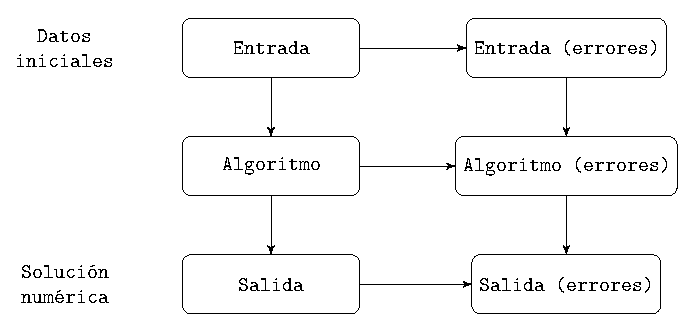
\includegraphics[scale=1]{dibujometodonum.eps} 
\end{figure}
\end{frame}
\begin{frame}
La solución obtenida por un método numérico es \textcolor{blue}{aproximada}, es decir, hay cierta diferencia entre la solución exacta y la solución numérica.
\end{frame}
\begin{frame}
\frametitle{Principales causas de la diferencia}
\begin{itemize}[<+->]
\item Falta de correspondencia entre el problema (modelo) matemático y el fenómeno físico real.
\item Errores en los datos iniciales (parámetros de entrada).
\item Errores en el método numérico usado para resolver el problema.
\item Errores de redondeo en las operaciones aritméticas.
\end{itemize}
\end{frame}
\subsection{Modelos y métodos numéricos}
%\section{\texorpdfstring{this is a very long title I \\ want to}{want to break manually}}
\begin{frame}
\frametitle{Conceptos en métodos numéricos}
\begin{itemize}[<+->]
\item Aproximación.
\item Estabilidad.
\item Convergencia.
\end{itemize}
\end{frame}
\begin{frame}
\frametitle{Aproximación}
Es la proximidad de un modelo numérico al modelo original (diferencial, integral, etc.) o el
grado de aproximación, caracteriza el error que se introduce al hacer discreto el modelo
continuo.
\\
\bigskip
El grado de aproximación $n$ se estima mediante un factor que tiene el error entre dos modelos.
\end{frame}
\begin{frame}
\frametitle{Estabilidad}
\begin{itemize}[<+->]
\item Caracteriza la manera de propagación de los errores iniciales dentro del algoritmo en el
proceso del cálculo.
\item Si el incremento de errores iniciales es considerable y sin ningún control, entonces el
método numérico se llama \textcolor{red}{inestable}.
\item Si los errores de cálculos dependen continuamente de los errores iniciales, entonces el método se llama \textcolor{blue}{estable}.
\end{itemize}
\end{frame}
\begin{frame}
\frametitle{Convergencia}
\begin{itemize}
\item  Significa que la solución numérica converge hacia la solución exacta cuando el tamaño de la malla $h$ tiene a cero, o el número de truncación $N$ tiende al infinito.
\end{itemize}
\end{frame}
\section{Errores en los métodos numéricos}
\frame{\tableofcontents[currentsection, hideothersubsections]}
\subsection{Tipos de errores}
\begin{frame}
\frametitle{Tipos de errores en los métodos numéricos}
\begin{itemize}[<+->]
\item \textcolor{brown}{Truncamiento}: se debe a las aproximaciones utilizadas en la fórmula
matemática del modelo.
\item \textcolor{orange}{Redondeo}: se asocia al hecho de que la representación de un número en la computadora se hace con un conjunto limitado de dígitos.
\end{itemize}
\end{frame}
\subsection{Series de Taylor}
\begin{frame}
\frametitle{Series de Taylor}
\begin{itemize}[<+->]
\item Las soluciones numéricas son en su mayoría, aproximaciones de las soluciones exactas.
\item Gran parte de los métodos numéricos se basan en la aproximación de funciones por medio de polinomios.
\end{itemize}
\end{frame}
\begin{frame}
\frametitle{Series de Taylor}
El desarrollo de Taylor es una serie infinita de potencias, representa de manera exacta a una función dentro de un cierto radio alrededor de un punto dado.
\\
\medskip
Al comparar el desarrollo polinomial de la solución numérica con la serie de Taylor de la solución exacta, es posible evaluar el error, conocido como error de \textcolor{blue}{truncamiento}.
\end{frame}
\begin{frame}
\frametitle{Serie de Taylor truncada}
Si se ignoran todos los términos de la serie de Taylor, excepto algunos cuantos, se puede obtener un polinomio que se aproxime a la función verdadera.
\\
\medskip
A éste polinomio se le llama \textit{serie de Taylor truncado} y se usa como punto de partida para obtener métodos numéricos.
\end{frame}
\begin{frame}
\frametitle{Definición de Serie de Taylor}
Una función $f(x)$ es analítica en $x=a$ si $f(x)$ se puede representar por medio de una serie de potencias en términos de $h = x-a$ dentro de un radio de convergencia $D > |x-a|> 0$.
\\
\bigskip
\pause
Una condición necesaria para que una función sea analítica es que todas sus derivadas sean continuas tanto en $x=a$ como en alguna vecindad alrededor de ese punto.
\end{frame}
\begin{frame}
\frametitle{Punto analítico}
Un punto en donde una función $f(x)$ no es analítica recibe el nombre de \emph{punto singular}. 
\\
\medskip
\pause
Si $f(x)$ es diferenciable en todas las partes de la vecindad de $x_{0}$, excepto en $x_{0}$ , entonces $x_{0}$ es un punto singular.
\\
\medskip
Los polinomios son analíticos en todas partes.
\end{frame}
\begin{frame}
\frametitle{Serie para una función análitica}
Si $f$ es analítica alrededor de $x = a$, se puede representar $f(x$) de manera exacta en la
vecindad de $x = a$ por medio de una serie de Taylor, dada por:
\fontsize{14}{14}\selectfont
\[ \begin{split} 
f(x) = f(a) + h \: f^{\prime}(a) + \dfrac{h^{2}}{2} \: f^{\prime \prime}(a) + \dfrac{h^{3}}{6} \: f^{\prime \prime \prime}(a) + \ldots \\
+ \ldots + \dfrac{h^{m}}{m!} \: f^{m}(a) + \ldots
\end{split}
\]
\end{frame}
\begin{frame}
\frametitle{Unicidad de la serie}
La serie de Taylor es única, esto quiere decir que no existe otra serie de potencias en $h = x-a$ para representar $f(x)$
\\
\bigskip
El desarrollo de Taylor de una función alrededor de $x = 0$ recibe el nombre de serie de Maclaurin.
\end{frame}
\begin{frame}
\frametitle{Truncamiento necesario}
En aplicaciones prácticas, se debe de truncar la serie de Taylor después cierto orden, ya que es imposible incluir un número infinito de términos. Si la serie se trunca después del término $N$, se expresa por:
\[ \begin{split} f(x) &= f(a) + hf'(a) + \dfrac{h^{2}}{2} f''(a) + \dfrac{h^{3}}{6} f'''(a) + \ldots \\
&= + \ldots + \dfrac{h^{N}}{N!} f^{N}(a) + O(h^{N+1}) 
\end{split} \]
\end{frame}
\begin{frame}
\frametitle{Truncamiento necesario}
\[ \begin{split} f(x) &= f(a) + hf'(a) + \dfrac{h^{2}}{2} f''(a) + \dfrac{h^{3}}{6} f'''(a) + \ldots \\
&= + \ldots + \dfrac{h^{N}}{N!} f^{N}(a) + O(h^{N+1}) 
\end{split} \]
Donde $h=x-a$ y $O(h^{N+1})$ representa el error por el truncamiento de los términos de orden $N+1$
\end{frame}
\begin{frame}
\frametitle{Error por el truncamiento}
El error global se puede representar como:
\[O(h^{N+1}) = f^{N+1}(a + \xi h) \dfrac{h^{N+1}}{(N+1)!} \hspace{1cm} 0 \leq \xi \leq 1\]
Dado que $\xi$ no puede calcularse con exactitud, se aproxima el término del error, haciendo $\xi = 0$
\[ O(h^{N+1}) \simeq f^{N+1}(a) \dfrac{h^{N+1}}{(N+1)!}\]
\end{frame}
\begin{frame}
\frametitle{Error por el truncamiento}
Si $N=1$ la serie de Taylor truncada es:
\[f(x) \simeq f(a) + f'(a) h \hspace{1cm} h=x-a\]
incluyendo el efecto del error, tenemos que
\[f(x) \simeq f(a) + f'(a) h + O(h^{2}) \]
donde
\[O(h^{2}) \simeq f''(a+ \xi h) \dfrac{h^{2}}{2} \hspace{1cm} 0 \leq \xi \leq 1\]
\end{frame}
% \begin{frame}
% \frametitle{Redondeo con \python.}
% \renewcommand*{\arraystretch}{2.5}
% \begin{center}
% %\captionof{table}{Funciones matemáticas intrínsecas}.
% \begin{longtable}{| l | l |}
% \hline
% Función & Resultado \\ \hline
% \endhead
% \texttt{ceil (x)} & \TitleParbox{Redondea al valor entero mayor más cercano a $x$.} \\ \hline
% \texttt{floor (x)} & \TitleParbox{Redondea al valor entero menor más cercano a $x$.} \\ \hline
% \texttt{round (x [, n])} &  \TitleParbox{Devuelve el valor de $x$ redondeado a $n$ dígitos desde el punto decimal.} \\ \hline
% \end{longtable}
% \end{center}
% \end{frame}
% \begin{frame}[fragile]
% \frametitle{Ejemplo con el código}
% \begin{lstlisting}[columns=fullflexible]
% from math import ceil, floor, pi

% a = 10.4563

% print('El valor de ceil(', a ,') es: ', ceil(a))

% print('El valor de floor(', a ,') es: ', floor(a))

% print('El valor de round(', a ,') es: ', round(a,3))

% print('El valor de round(', pi ,',3) es: ', round(pi,3))
% \end{lstlisting}
% \end{frame}
\section{Los números en las computadoras}
\frame{\tableofcontents[currentsection, hideothersubsections]}
\subsection{Base decimal}
\begin{frame}
\frametitle{Representación en una computadora}
Antes de lanzarnos a la revisión de estrategias de solución para un problema real, se requiere entender las limitaciones que tendremos para representar los números en una computadora.
\end{frame}
\begin{frame}
\frametitle{De lo continuo a la discreto}
Hemos recibido una formación matemática en donde lo común es pensar en intervalos continuos.
\\
\bigskip
\pause
Donde hemos logrado demostrar que existe un conjunto infinito de valores dentro de un intervalo finito.
\end{frame}
\begin{frame}
\frametitle{De lo continuo a lo discreto}
Pero en la práctica con las computadoras, no podremos representar esa continuidad.
\\
\bigskip
\pause
Tendremos que \enquote{truncar} nuestra representación, ya que el hardware que usamos no nos permite contar con esa propiedad de continuidad.
\end{frame}
\begin{frame}
\frametitle{Base decimal}
El valor decimal de un número de base $r$ es
\[(abcdefg.hijk)_{r}\]
que se calcula como:
\begin{eqnarray*}
ar^{6} + br^{5} + cr^{4} + dr^{3} + er^{2} + fr +
 g + {} \\
{} + hr^{-1} + ir^{-2} + jr^{-3} + kr^{-4}
\end{eqnarray*}
\end{frame}
\begin{frame}
\frametitle{Un número real en la computadora}
La menor y mayor magnitud de un número real que se pueden representar en una computadora, varían de acuerdo con el diseño tanto de hardware como de software.
\\
\bigskip
Los números reales en una computadora no son continuos. Si nos fijamos en número cercano a cero, el número positivo más pequeño en una IBM es $2.9 \times 10^{-39}$
\end{frame}
\begin{frame}
\frametitle{Un número real en la computadora}
Por tanto, no se pueden representar números entre $0$ y $2.9 \times 10^{-39}$ 
\\
\bigskip
A éste intervalo se le conoce como \textcolor{blue}{épsilon de la máquina}.
\end{frame}
\subsection{Epsilon de la máquina}
\begin{frame}
\frametitle{Epsilon de la máquina}
Hay dos maneras de definir el épsilon de la máquina: \textcolor{red}{un épsilon absoluto} y un \textcolor{blue}{épsilon relativo}.
\\
\bigskip
Este último es el más usado, ya que el conjunto de números en la computadora es finito.
\end{frame}
\begin{frame}
\frametitle{Epsilon relativo de la máquina}
Definición de épsilon relativo:
\[ \epsilon_{maq} = \epsilon = \min[t>0 : 1+t>1 ] \]
\end{frame}
\begin{frame}
\frametitle{Epsilon absoluto de la máquina}
El épsilon absoluto se define comparando con cero:
\[ \epsilon_{abs} = \min[t>0 : t \neq 0] \]
\textcolor{blue}{En realidad el épsilon depende de la máquina pero también del sistema operativo, del compilador y del tipo de números utilizados.}
\end{frame}
\begin{frame}
\frametitle{Números reales en un computadora}
Para una computadora IBM PC tenemos:
\fontsize{10}{10}\selectfont
\begin{figure}
\centering
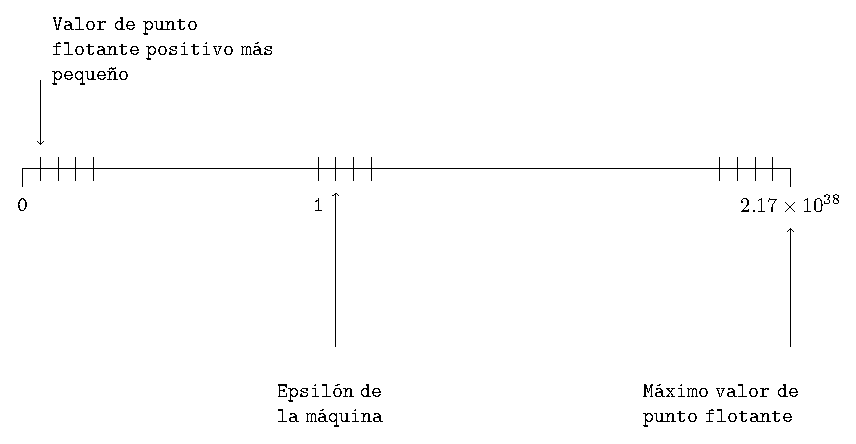
\includegraphics[scale=0.8]{epsilonmaquina.eps}
\end{figure}
\end{frame}
\begin{frame}[fragile]
\frametitle{Calculemos el épsilon con \python}
Una manera sencilla de calcular el épsilon del equipo que estamos usando, es reducir a la mitad un intervalo inicial, hasta cierto punto.
\\
\bigskip
\pause
Empecemos dividiendo a la mitad la unidad.
\begin{figure}
\centering
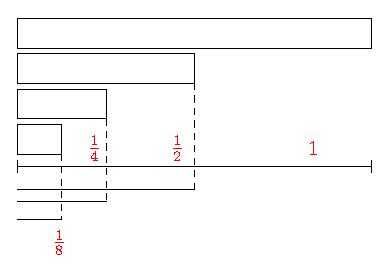
\includegraphics[scale=1]{epsilonmaquina_02.eps}
\end{figure}
\end{frame}
\begin{frame}[fragile]
\frametitle{Calculemos el epsilón con \python}
\begin{lstlisting}[caption=Código para el épsilon, basicstyle=\linespread{1.2}\ttfamily\small, columns=fullflexible]
t = 1.0;
while 1+t != 1:
  eps = t
  t = t/2
print ('el epsilon de la maquina es: ', eps)
\end{lstlisting}
\end{frame}
% \begin{frame}
% \frametitle{Error de truncamiento}
% Se originan al emplear al número finito de términos para calcular un valor que requiere un número infinito de términos.
% \\
% \bigskip
% Por ejemplo, una expresión que permite determinar de forma exacta el valor del número de Euler (base de los logaritmos naturales) a través de una serie de MacLaurin es:
% \[ e^{x} = \sum \dfrac{x_{i}}{i!}\]
% \end{frame}
% \begin{frame}
% Sin embargo, una aproximación a dicho valor, puede obtenerse a través de su expresión finita:
% \[ e^{x} \simeq \sum_{i=0}^{k} \dfrac{x_{i}}{i!} \hspace{1cm} k<\infty \]
% Es claro que esta expresión finita es manejable computacionalmente hablando, al contrario que la fórmula expresada en su forma infinita.
% \end{frame}
% \begin{frame}
% \frametitle{Error por redondeo}
% Se origina por el hecho de que una computadora sólo puede representar un número finito de
% términos. Para expresar una cantidad con un desarrollo decimal infinito, se tiene que prescindir de la mayoría de ellos.
% \\
% \bigskip
% Por ejemplo, el número $\pi = 3.14159265 \ldots$, tiene un desarrollo decimal infinito no periódico. Por lo tanto, para fines de cálculo, sólo se toman algunos de sus dígitos.
% \end{frame}
% \begin{frame}
% \frametitle{Estrategias}
% \begin{itemize}[<+->]
% \item \textcolor{blue}{Redondeo}. Prescinde de cierto número de cifras significativas y realiza un ajuste, sobre la última cifra no descartada: $\pi = 3.1416$
% \item \textcolor{red}{Corte o poda}: Prescinde de cierto número de cifras significativas sin realizar un ajuste sobre la última cifra no descartada: $\pi = 3.1415$
% \end{itemize}
% \end{frame}
\section{Tipos de errores}
\frame{\tableofcontents[currentsection, hideothersubsections]}
\subsection{Errores en programación}
\begin{frame}
\frametitle{Los errores}
Como ya hemos mencionado que un programa numérico ejecutado en la computadora, nos va a devolver un resultado que es una aproximación, entonces hay que considerar que existe un \textcolor{red}{error} debido al proceso.
\end{frame}
\begin{frame}
\frametitle{Los errores}
En métodos numéricos es importante identificar el tipo de error que se obtiene, ya que nos permitirá entonces establecer no sólo un valor, sino la magnitud del error comparada con el valor esperado o \enquote{exacto}.
\end{frame}
\begin{frame}
\frametitle{Nuevos conceptos}
El error entendido como la suma o consecuencia por un truncamiento o redondeo, se clasifica en:
\begin{itemize}[<+->]
\item \textcolor{red}{Error absoluto verdadero}.
\item \textcolor{orange}{Error relativo verdadero}.
\item \textcolor{blue}{Error relativo aproximado}.
\end{itemize}
\end{frame}
\subsection{Error absoluto verdadero}
\begin{frame}
\frametitle{Error absoluto verdadero}
Supóngase que $\widehat{p}$ es una aproximación a p.
\\
\bigskip
El error absoluto verdadero se define con la siguiente expresión:
\[ E_{v} = \vert p - \widehat{p} \vert \]
Esta definición de error, lo cuantifica en términos brutos.
\end{frame}
\begin{frame}
\frametitle{Tamaño del error}
 No obstante, una medida que puede describir con mayor detalle o proporción el error, es aquella que lo expresa en términos porcentuales.
 \\
 \bigskip
 Para ello se emplea el error verdadero relativo.
\end{frame}
\subsection{Error relativo verdadero}
\begin{frame}
\frametitle{Error relativo verdadero}
Supóngase que $\widehat{p}$ es una aproximación a p. El error relativo verdadero se calcula con la siguiente expresión:
\[ e_{v} = \dfrac{\vert p - \widehat{p} \vert }{p}\]
El resultado suele expresarse en términos porcentuales.
\end{frame}
\subsection{Error relativo aproximado}
\begin{frame}
\frametitle{Error relativo aproximado}
El error relativo aproximado, mide el error de un método numérico, determinando el error de la iteración actual respecto el error surgido en la iteración anterior:
\[ e_{a} = \dfrac{\vert \widehat{x}_{i} - \widehat{x}_{i-1} \vert}{\widehat{x}_{i}}\]
Donde $x_{i}$ es la aproximación actual a $x$ y 
$x_{i-1}$ es la aproximación anterior a $x$.
\end{frame}
\begin{frame}
\frametitle{Tolerancia}
En métodos numéricos suele establecerse una tolerancia porcentual como criterio de paro, tal
que el error relativo aproximado de un método, no exceda dicha tolerancia.
\[ e_{a} < t \]
donde $t$, es tolerancia fijada de antemano.
\end{frame}
\begin{frame}
\frametitle{Tolerancia}
A menor tolerancia se tiene mayor precisión en la aproximación al valor verdadero, sin embargo esto implica un aumento en el número de iteraciones requeridas para detener el método.
\end{frame}
\section{Contaminación en los cálculos}
\begin{frame}
\frametitle{Contaminación en los cálculos.}
Un error en un cálculo numérico \enquote{contamina} las sucesivas evaluaciones.
\\
\bigskip
Esta propagación puede describirse en términos de dos conceptos relacionados: los de estabilidad y condición.
\end{frame}
\subsection{Condición}
\begin{frame}
\frametitle{Condición}
La condición de una función $f(x)$ mide la sensibilidad de los valores de $f(x)$ a pequeños
cambios de $x$, se define como:
\[ C = \left | \dfrac{E_{rel} (f(x))}{E_{rel}(x)} \right |  \]
\end{frame}
\begin{frame}
\frametitle{Definición de condición}
Del teorema del valor medio en cálculo, podemos expresar
\[ \begin{split} f(x_{T}) - f(x_{A}) & \approx f'(x_{t})(x_{T} - x_{A}) \rightarrow E_{rel}(f(x)) \approx \\ 
 & \approx \dfrac{f'(x_{T})}{f(x_{T})} (x_{T} - x_{A}) \end{split} \]
luego
\[ C \approx \left | x_{T} \dfrac{f'(x_{T})}{f(x_{T})} \right | \]
\end{frame}
\begin{frame}
\frametitle{Definición de condición}
Se utilizará ésta definición como definición de condición para funciones $f(x)$ de una variable real.
\\
\bigskip
Entonces los números de condición serán
\[ C = \left | x \dfrac{f'(x)}{f(x)} \right | \]
\end{frame}
\begin{frame}
\frametitle{Definición de condición}
\[ C = \left | x \dfrac{f'(x)}{f(x)} \right | \]
\setbeamercolor{item projected}{bg=red!70!black,fg=white}
\setbeamertemplate{enumerate items}[circle]
\begin{enumerate}[<+->]
\item Para un $x$ dado $0 < C(x) < 1$ se dirá que el problema está bien condicionado, y cuanto menor sea $C$, mejor condicionado.
\item Si $C(x) > 1$, el problema estará mal condicionado.
\item Si $C(x) = 1$, el error relativo se mantiene.
\end{enumerate}
\end{frame}
\begin{frame}
\frametitle{Ejemplos}
 Las siguientes funciones están bien condicionadas?
\begin{enumerate}
\item $f(x) = \sqrt{x} \hspace{1.5cm} C(x) = ?$
\item $g(x) = x^{2}-1 \hspace{1.5cm} C(x) = ?$
\end{enumerate}
\end{frame}
\subsection{Estabilidad}
\begin{frame}
\frametitle{Estabilidad}
La estabilidad de un algoritmo describe la sensibilidad de un método numérico específico
respecto a los inevitables errores de redondeo cometidos durante su ejecución en aritmética de precisión finita.
\end{frame}
\begin{frame}
\frametitle{Estabilidad}
Consideremos la siguiente función:
\[ f(x) = \sqrt{x+1} - \sqrt{x} \]
Su número de condición es:
\[ C(x) = \left | x \dfrac{f'(x)}{f(x)} \right | = \dfrac{x}{2 \sqrt{x} \sqrt{x+1}}\]
Vemos que $C(x)< \frac{1}{2}$ para $x>0$, por lo que la función está bien condicionada pero ...
\end{frame}
\begin{frame}
\frametitle{Estabilidad}
El pseudo-código para calcular $x$ de tal forma que se vayan realizando las operaciones, es:
\setbeamercolor{item projected}{bg=red!70!black,fg=white}
\setbeamertemplate{enumerate items}[circle]
\begin{enumerate}[<+->]
\item obtener $x$
\item $y = x + 1$
\item $f = sqrt(y)$
\item $g = sqrt(x)$
\item $h = f-g$
\end{enumerate}
\pause
es inestable para $x$ grandes, dado el paso 5, por lo que debemos de re-estructurar la función.
\end{frame}
\subsection{Eficiencia}
\begin{frame}
\frametitle{Eficiencia}
\emph{Debemos evitar que todo algoritmo sea inestable}. 
\\
\bigskip
Si existieran varios métodos para evaluar una misma función, entonces conviene utilizar aquel que sea más eficiente, es decir, más rápido.
\end{frame}
\begin{frame}
\frametitle{Eficiencia}
\textcolor{blue}{Hay que aprovechar al máximo los recursos: hardware, software, algoritmos, para resolver problemas más complejos y no para resolver peor problemas simples.}
\end{frame}
\begin{frame}
\frametitle{Ejemplo de eficiencia}
Por ejemplo, para calcular $x**4$ para un $x$ dado, no es buena idea calcular $x**4.0$ (exponente en punto flotante).
\\
\bigskip
\pause
La mejor idea consiste en economizar el cálculo en dos pasos:
\begin{eqnarray*}
x2 &=& x*x \\
x4 &=& x2*x2
\end{eqnarray*}
y no un producto 
\[ x4=x*x*x*x \]
\end{frame}
\begin{frame}
\frametitle{Ejemplo: Evaluación de polinomios}
Supongamos que queremos evaluar el polinomio:
\[ P(x) = 2 + 4x - 5 x^{2} + 2 x^{3} - 6 x^{4} + 8 x^{5} + 10 x^{6}\]
\pause
Contando con que cada potencia de exponente $k$ entero como $k-1$ productos, tendríamos que el total de productos para evaluar en forma directa es:
\[ 1+2+3+4+5+6=21\]
Además de seis sumas.
\end{frame}
\begin{frame}
\frametitle{Ejemplo: Evaluación de polinomios}
Una mejora en el algoritmo , es calcular primero las potencias de forma sucesiva:
\begin{eqnarray*}
x^{2} & = & x*x \\
x^{3} & = & x*x^{2} \\
x^{4} & = & x*x^{3} \\
x^{5} & = & x*x^{4} \\
x^{6} & = & x*x^{5}
\end{eqnarray*}
De tal forma que se añade un producto por cada potencia, para un total de productos:
\[1+2+2+2+2+2=11\]
\end{frame}
\begin{frame}
\frametitle{Ejemplo: Evaluación de polinomios}
Con el polinomio
\[ P(x)=2 + 4 x - 5 x^{2} + 2 x^{3} - 6 x^{4} + 8 x^{5} + 10 x^{6}\]
podemos mejorar el algoritmo de la siguiente manera
\fontsize{12}{12}\selectfont
\[ P(x) = 2 + x \left\lbrace 4 + x \left( -5 + x \left[ 2 + x \left(-6 +x \left\lbrace 8+x*10 \right\rbrace \right) \right] \right) \right\rbrace  \]
\end{frame}
\begin{frame}
\frametitle{Ejemplo: Evaluación de polinomios}
Para evaluar un polinomio de grado $n$ en el que ninguno de los coeficientes es cero, se necesitan
\\
\medskip
\pause
\begin{tabular}{l l}
$\dfrac{n(n+1)}{2}$ & Productos para el primer método \\
$2n-1$ & para el segundo métodos \\
$n$ & para el tercero
\end{tabular}
\\
\medskip
\pause
Antes de escribir una línea de código, hay que revisar la manera en que podemos optimizar la solución del problema.
\end{frame}
\section{Algoritmo de Horner}
\begin{frame}
\frametitle{Algoritmo de Horner}
Dado el polinomio
\[ P(x) = a_{0} + a_{1} x + \ldots + a_{n} x^{n} \hspace{1cm} a_{n} \neq 0 \]
\pause
La evaluación de $P(x)$ para cierto valor de $x=z$ se puede realizar en $n$ pasos mediante:
\begin{eqnarray*}
b_{n} &=& a_{n} \\
b_{n-1} &=& a_{n-1} + z*b_{n} \\
b_{n-2} &=& a_{n-2} + z*b_{n-1} \\
\vdots \\
b_{0} &=& a_{0}+z*b_{1}
\end{eqnarray*}
\end{frame}
\begin{frame}
\frametitle{Pseudocódigo}
\setbeamercolor{item projected}{bg=red!70!black,fg=white}
\setbeamertemplate{enumerate items}[circle]
\begin{enumerate}[<+->]
\item $b_{n} = a_{n}$
\item repetir mientras $n>0$
\item $n = n-1$
\item $b=a_{n}+z*b$
\item volver al paso 2
\item $p(z)=b$
\end{enumerate}
\end{frame}
\begin{frame}
\frametitle{Evalúa el polinomio $P(x)$}
\[ P(x)=2 + 4 x - 5 x^{2} + 2 x^{3} - 6 x^{4} + 8 x^{5} + 10 x^{6}\]
\\
\medskip
\begin{center}
\begin{tabular}{S | c}
$x$ & $P(x)$ \\
\hline -1.5 & \\
\hline -0.65 & \\
\hline 0.1 & \\
\hline 1.4 & \\
\hline 2.87 & 
\end{tabular}
\end{center}
\end{frame}
\begin{frame}
\frametitle{Resultado}
El polinomio $P(x)$ evaluado con el método de Horner:
\\
\medskip
\begin{center}
\begin{tabular}{S[table-format=1.2] | S[table-format=4.5] }
%x & P(x) \\
\hline -1.5 & 0.78125 \\
\hline -0.65 & -4.50683 \\
\hline 0.1 & 2.35149 \\
\hline 1.4 & 98.55968 \\
\hline 2.87 & 6758.70245
\end{tabular}
\end{center}
\end{frame}
\begin{frame}
\frametitle{Extendiendo la respuesta al problema}
¿Cómo resolver el problema usando una función? ¿mostrando una tabla con formato de salida? usando una gráfica que muestre $P(x)$ y un conjunto de datos evaluados? ¿Evaluar el error relativo?
\end{frame}
\begin{frame}
\frametitle{Extendiendo la respuesta al problema}
Ya contamos con las herramientas necesarias para extender la respuesta al problema, en nuestro código podemos agregar funciones, ajustar formatos de salida en los resultados, graficar el polinomio y los puntos (o un conjunto diferente de puntos), y obtener el error relativo.
\end{frame}
\begin{frame}
\frametitle{Pasos a resolver}
\setbeamercolor{item projected}{bg=red!70!black,fg=white}
\setbeamertemplate{enumerate items}[circle]
\begin{enumerate}[<+->]
\item Conviene definir una función que resuelva la evaluación del método de Horner.
\item Para obtener el error relativo, se debe de evaluar el polinomio y considerar que los valores obtenidos, son los valores exactos.
\item Comparamos los resultados mediante una gráfica que represente los dos resultados de la evaluación.
\end{enumerate}
\end{frame}
\begin{frame}[fragile]
\frametitle{Resultado gráfico más completo}
En la gráfica se muestra un conjunto de datos que se evalúan y posteriormente con la función (en línea continua) se compara, podemos ver que los resultados son prácticamente los mismos.
\begin{figure}
	\centering
	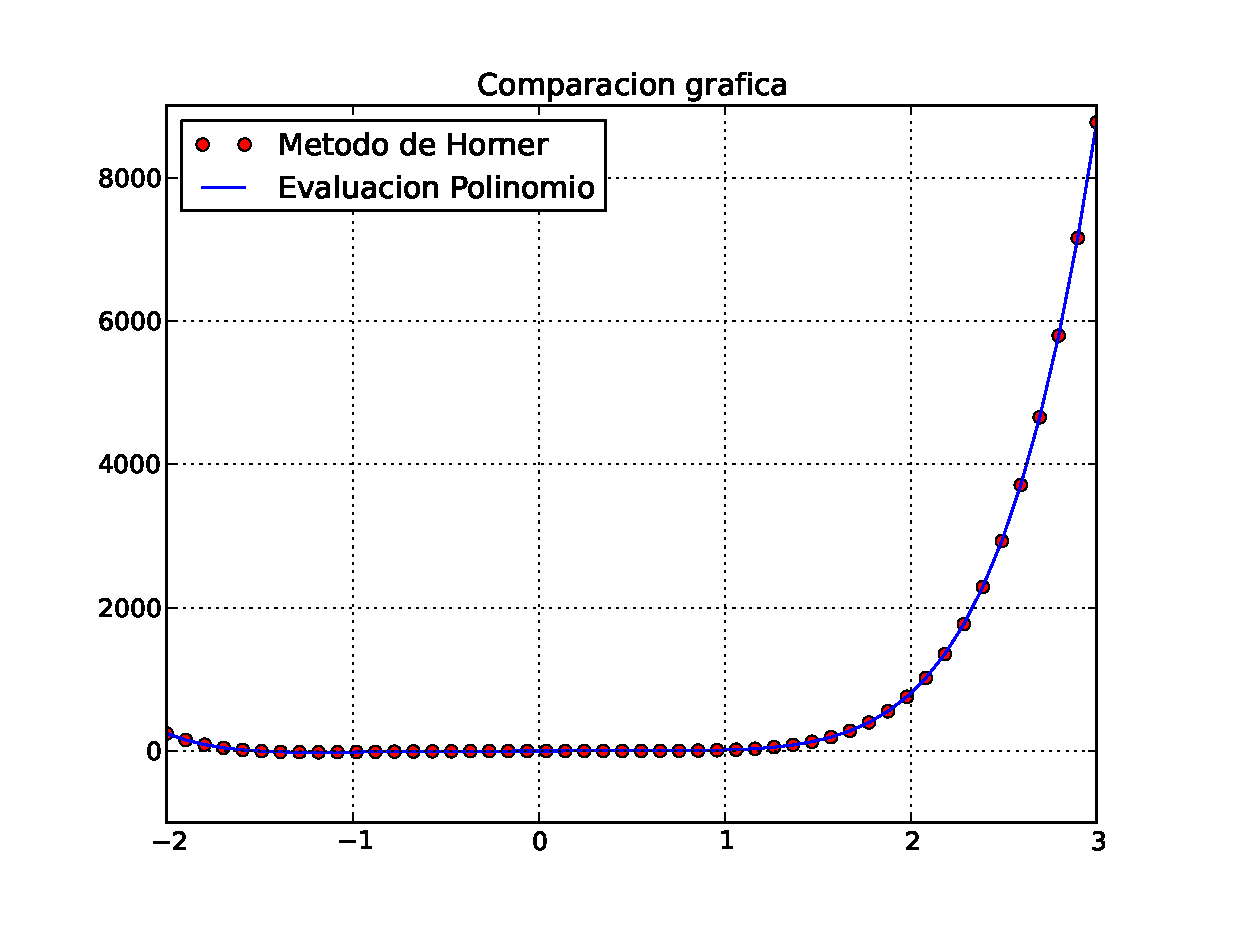
\includegraphics[scale=0.35]{MetodoHorner.eps} 
\end{figure}
\end{frame}
\begin{frame}[fragile]
\frametitle{Estructuramos el código en \python.}
Definimos mediante dos listas:
\setbeamercolor{item projected}{bg=red!70!black,fg=white}
\setbeamertemplate{enumerate items}[circle]
\begin{enumerate}
\item Los valores donde queremos evaluar el polinomio $P(x)$.
\item Los coeficientes de $P(x)$.
\end{enumerate}
\end{frame}
\begin{frame}[fragile]
\frametitle{Función de Horner.}
\fontsize{14}{14}\selectfont
\begin{lstlisting}[caption=Código para la función de Horner, basicstyle=\linespread{1.2}\ttfamily\small, columns=fullflexible]
# Metodo de Horner

def P_Horner(x):
    P_Hor=0
    for n in range(len(a)-1,-1,-1):     
        P_Hor=a[n]+P_Hor*x
    return P_Hor
\end{lstlisting}
\end{frame}
\begin{frame}[fragile]
\frametitle{Función que evalúa directamente $P(x)$.}
\fontsize{14}{14}\selectfont
\begin{lstlisting}[caption=Evaluación directa de la función, basicstyle=\linespread{1.2}\ttfamily\small, columns=fullflexible]
# Evaluacion directa

def P_Directo(x):
    return 2 + 4 * x - 5 * x**2 + 2 * x**3 -6 * x**4 + 8 * x**5 + 10 * x**6
\end{lstlisting}
\end{frame}
\begin{frame}[fragile]
\frametitle{Calculamos el error relativo.}
\fontsize{14}{14}\selectfont
\begin{lstlisting}[caption=Evaluación del error relativo, basicstyle=\linespread{1.2}\ttfamily\small, columns=fullflexible]
# Calculo de error relativo

def Err_Rel(p,p_): return (p-p_)/p*100
    
\end{lstlisting}
\end{frame}
\begin{frame}[fragile]
\frametitle{Uso de valores conocidos}
\begin{lstlisting}[caption=Valores conocidos, basicstyle=\linespread{1.2}\ttfamily\small, columns=fullflexible]
# Valores de x0 para evaluar P(x0)
x0 = [-1.5, -0.65, 0.1, 1.4, 2.87]

# Coeficientes a de P(x)
a = [2,4, -5, 2, -6, 8, 10]
\end{lstlisting}
\end{frame}
\begin{frame}[fragile]
\frametitle{Mostramos el error relativo de los puntos a evaluar.}
\fontsize{14}{14}\selectfont
\begin{lstlisting}[caption=Error relativo calculado, basicstyle=\linespread{1.2}\ttfamily\small, columns=fullflexible]
# Evaluacion de valores de P(x0)

for i in range(len(x0)):                 
    print ("P(%.2f) =" %x0[i],P_Horner(x0[i]), "; Error rel. =", Err_Rel(P_Directo(x0[i]),P_Horner(x0[i])))
\end{lstlisting}
\end{frame}
\begin{frame}[allowframebreaks, fragile]
\frametitle{Los resultados en una gráfica.}
\fontsize{14}{14}\selectfont
\begin{lstlisting}[caption=Elaboración de la gráfica, basicstyle=\linespread{1.2}\ttfamily\small, columns=fullflexible]
import matplotlib.pyplot as plt
import numpy as np

x = np.linspace(-2., 3.)

plt.plot(x,P_Horner(x),'ro', label='Metodo de Horner')

plt.plot(x,P_Directo(x), label='Evaluacion Polinomio')

plt.title('Comparacion grafica')
plt.legend(loc='upper left')

plt.grid(True)
plt.show()
\end{lstlisting}
\end{frame}
\begin{frame}\frametitle{Función para generar secuencia de reales}
Ya hemos mencionado que la librería \funcionazul{numpy} extiende el conjunto de funciones matemáticas que se tienen dentro de la otra librería \funcionazul{math}.
\\
\bigskip
Veamos la sintaxis de la función \funcionazul{linspace} que aparece en la rutina de graficación.
\end{frame}
\begin{frame}
\frametitle{La función \texttt{linspace}}
Sintaxis mínima:
\\
\medskip
\texttt{linspace(inicio, fin, num=50)}
\\
\medskip
Donde:
\begin{itemize}
\item \texttt{inicio}: es el valor a partir del cual queremos generar la secuncia de puntos.
\item \texttt{fin}: es el valor en donde se detiene la secuencia de puntos.
\item \texttt{num}: es el número de puntos que se genera en el intervalo, por defecto se generan 50 puntos.
\end{itemize}
\end{frame}
\begin{frame}
\frametitle{La secuncia que se genera}
Lo que obtenemos con \funcionazul{linspace}, es una secuencia de puntos distribuidos uniformemente en el intervalo \texttt{[inicio, fin]}.
\end{frame}
\end{document}
